
L'obiettivo di questo elaborato è progettare ed implementare una soluzione che consenta la distribuzione di applicazioni nel panorama dell'Edge-Cloud continuum. Le applicazioni devono essere sviluppate seguendo il paradigma FaaS ed essere in grado di funzionare indipendentemente dall'infrastruttura sottostante e senza essere ri-compilate. Inoltre, la piattaforma deve essere in grado di effettuare migrazioni live delle applicazioni e spostare il carico computazionale in modo automatico in risposta a problemi infrastrutturali o a necessità di bilanciamento del carico. La migrazione deve avvenire anche fra ambienti eterogenei, per esempio deve essere possibile spostare l'esecuzione di un'applicazione da un nodo Edge ad uno Cloud.\\
Le applicazioni in esecuzione devono poter interagire e scambiarsi informazioni, quindi c'è necessità di utilizzare un sistema di messaggistica distribuito che si sposi con il modello di esecuzione ad eventi del paradigma FaaS.\\

Per facilitare l'adozione del paradigma FaaS è stato scelto un modello applicativo basato sui microservizi\cite{Aksakalli2021Deployment}, in particolare facente uso della tecnologia Wasm. La scelta è stata fatta in quanto riesce a superare una criticità associata alla tradizionale soluzione del container. Essi infatti vengono eseguiti in runtime strettamente collegati al kernel del sistema operativo in cui risiedono ed esso cambia con l'architettura della macchina. Questo costringerebbe ad avere una versione dell'applicazione per ogni architettura supporata.\\
Le applicazioni compilate in Wasm invece possono operare in qualsiasi host senza preoccuparsi di requisiti 
infrastrutturali, consentendo l'utilizzo dello stesso artifact per ogni host (come mostrato nella Figura \ref{fig:modello_edge_computing}).\\

\FloatBarrier
\begin{figure}[h]
    \centering
    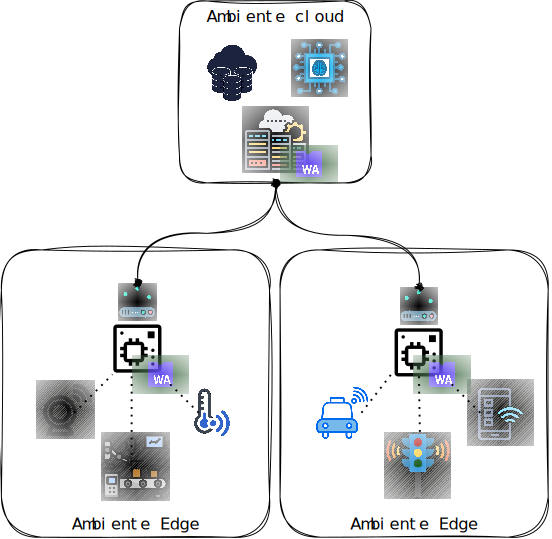
\includegraphics[width=0.8\textwidth]{img/schemi/schemi-Scenari.drawio.pdf}
    \caption{Modello Edge Computing}
    \label{fig:modello_edge_computing}
\end{figure}
\FloatBarrier

Per soddisfare i requisiti di migrazione e bilanciamento automatico fra nodi si è scelto di adottare wasmCloud, principalmente per i seguenti motivi:
\begin{itemize}
    \item Supporto all'esecuzione di componenti Wasm e specifica WASI Preview 2.
    \item Supporto sia di ambienti Cloud Native (come Kubernetes o Docker) che tradizionali (VM con Linux).
    \item Networking basato su rete mesh Lattice che consente di astrarre l'infrastruttura sottostante e permette l'interazione dei componenti.
    \item Cluster auto-rigenerante e facilmente scalabile all'interno del Lattice.
    \item Comunicazione efficiente grazie al backend basato su NATS.
    \item Gestione delle applicazioni tramite OCI Registry.
\end{itemize}

NATS è stata la soluzione selezionata anche per quanto riguarda la comunicazione e l'interazione delle applicazioni stesse, principalmente per il suo supporto alla clusterizzazione e alla distribuzione su ambienti edge basata su nodi Leaf.\\
L'infrastruttura completa può essere schematizzata come nella Figura \ref{fig:infra_wasmcloud_nats}.

\FloatBarrier
\begin{figure}[h]
    \centering
    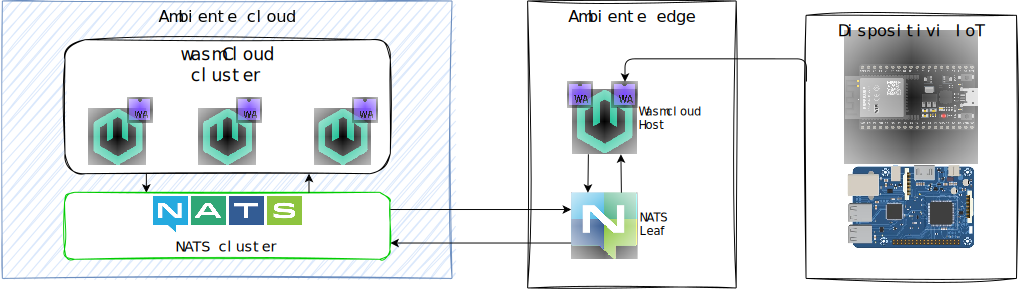
\includegraphics[width=\textwidth]{img/schemi/schemi-architettura-infra.drawio.pdf}
    \caption{Infrastruttura target}
    \label{fig:infra_wasmcloud_nats}
\end{figure}
\FloatBarrier

Il processo di trasformazione delle funzioni in componenti Wasm e la loro distribuzione verrà approfondita nella prossima sezione.

\section{PELATO Framework}

Lo scopo ultimo di questo elaborato è quindi trasformare una semplice funzione in un codice compilabile in componente Wasm, configurarlo in modo che possa essere deployato su ambienti wasmCloud e distribuirlo sull'infrastruttura.\\
La soluzione proposta è un framework denominato PELATO, acronimo di \textbf{Progettazione ed Esecuzione di Lifecycle Automatizzati e Tecnologie d'Orchestrazione per moduli WebAssembly}, che ha lo scopo di:

\begin{itemize}
    \item Fornire un modo intuitivo per istanziare un modulo FaaS, quindi ridurre al minimo le responsabilità dell'utilizzatore che dovrà esclusivamente specificare il codice della funzione da eseguire nella task remota.
    \item Consentire all'utilizzatore di configurare in modo intuitivo i metadati delle task, come il nome, il target di deployment, ma anche l'origine e la destinazione dei dati.
    \item Astrarre i più possibile il processo di generazione del codice e di Build del componente Wasm.
    \item Gestire il deployment dei componenti nell'infrastruttura.
\end{itemize}

Nelle seguenti sezioni verranno approfondite le scelte tecnologiche ed architetturali che sono state compiute durante la realizzazione di questo progetto.

\subsection{Tecnologie}

In questa sezione verranno elencate e spiegate le tecnologie utilizzate per lo sviluppo di questa soluzione. WebAssembly e gli argomenti correlati sono già stati ampiamente descritti nella sezione [\ref{sec:webassembly}], quindi ci concentreremo principalmente sui linguaggi e i tool utilizzati dal framework PELATO, come i linguaggi Python e Go.

\subsubsection{Python}

Il framework è stato implementato utilizzando Python, un linguaggio di programmazione ad alto livello interpretato ed orientato agli oggetti, apprezzato per la sua sintassi chiara e la tipizzazione dinamica che ne facilitano l'apprendimento e la manutenzione. Grazie a un vasto ecosistema di librerie è ampiamente utilizzato in ambiti come data science, sviluppo web e intelligenza artificiale. Supporta diversi paradigmi di programmazione e, grazie alla gestione automatica della memoria, riduce la complessità nello sviluppo. Inoltre, la sua portabilità su Windows, macOS e Linux lo rende adatto a molteplici contesti, dalla prototipazione rapida alle soluzioni enterprise.\\
È noto che Python, pur offrendo un ecosistema ricco e una sintassi intuitiva, può presentare limitazioni in termini di performance, soprattutto per operazioni CPU-intensive. Questo è in gran parte dovuto al Global Interpreter Lock (GIL), che impedisce l'effettivo sfruttamento del multi-threading in scenari di calcolo parallelo. Questi problemi sono stati risolti spostando il carico computazionale ed il parallelismo su strumenti esterni come Docker (la metodologia verrà spiegata in seguito).\\
La scelta di impiegare questo linguaggio per sviluppare il framework è stata motivata principalmente dalla vasta gamma di librerie disponibili. In particolare, per lo sviluppo di PELATO ce ne sono due fondamentali:
\begin{itemize}
    \item \textbf{Jinja}: è un motore di template per Python che permette di generare contenuti dinamici combinando testo statico e logica di programmazione. Utilizzato in framework web come Flask e strumenti di automazione come Ansible, trova applicazione anche nella configurazione di orchestratori come Helm, dove consente di parametrizzare file YAML. Attraverso la sintassi con doppie parentesi graffe, Jinja sostituisce variabili con valori definiti, rendendo la configurazione più flessibile e riutilizzabile. È stato utilizzato in fase di generazione del codice per parametrizzare lo stesso in base alla configurazione specificata dall'utente.
    \item \textbf{docker-py}: questa libreria consente di interagire con le API di Docker direttamente da Python, facilitando la gestione e l'automazione dei container. Permette operazioni come la creazione, l'avvio e l'eliminazione di container, oltre alla gestione di immagini e volumi. Questa integrazione è stata fondamentale per poter parallelizzare le operazioni di build e di deployment dei moduli Wasm.
\end{itemize}

\subsubsection{Golang}

Un altro linguaggio utilizzato è Go, noto anche come Golang, un progetto open source sviluppato da Google per offrire un equilibrio tra efficienza, sicurezza e semplicità. Grazie alla tipizzazione statica, al garbage collector e a un avanzato sistema di concorrenza basato sulle goroutine, Go consente la creazione di applicazioni scalabili e performanti. Pur supportando la programmazione orientata agli oggetti attraverso interfacce e struct, mantiene una sintassi essenziale e pragmatica. Inoltre, la sua ricca standard library fornisce strumenti per la gestione della rete, il parsing di file e la sicurezza crittografica.\\
Go è il linguaggio selezionato per la programmazione delle funzioni da eseguire nei componenti Wasm:
l'utente che utilizza il framework PELATO dovrà programmare i propri flussi utilizzando Go.\\
La scelta di utilizzare questo linguaggio è stata effettuata principalmente perché è uno dei due linguaggi (insieme a Rust) che attualmente implementa la specifica WASI Preview 0.2, necessaria per la composizione delle applicazioni tramite components e providers su wasmCloud.\\
La scelta di Go invece di Rust è avvenuta perché la sintassi di quest'ultimo risulta complessa e di difficile lettura, rendendolo meno accessibile per utenti senza esperienza pregressa. Al contrario, Go offre una sintassi più chiara e intuitiva, facilitando lo sviluppo e la manutenzione del codice.\\

\subsection{Struttura del framework}

In questa sezione verrà data una descrizione architetturale ad alto livello di PELATO. Il framework è sviluppato secondo un'architettura che adotta il pattern di progettazione \texttt{Facade} che fornisce un'interfaccia semplificata e unificata per accedere alle varie funzionalità. In pratica, una classe Facade funge da punto di accesso centrale, nascondendo la complessità interna e offrendo metodi di alto livello per interagire con il sistema.\\
La classe \texttt{Pelato} viene utilizzata come punto di accesso per la CLI (Command Line Interface), memorizza le configurazioni iniziali e si occupa di salvare le metriche. Inoltre è responsabile dell'esecuzione della logica di business implementata nei tre package:
\begin{itemize}
    \item \texttt{code\_generator}
    \item \texttt{wasm\_builder}
    \item \texttt{component\_deploy}
\end{itemize}

La configurazione iniziale della classe avviene tramite variabili d'ambiente (che possono essere caricate dal framework tramite un file \texttt{.env} locale, verranno dati più dettagli in seguito); ciò consente una facile implementazione del framework come applicazione containerizzata, nel caso si volesse ``trasformare" in un servizio gestito in Cloud.\\
Questo pattern di progettazione aumenta la modularità dei componenti facilitando eventuali estensioni, come quella mostrata nella Figura \ref{fig:pelato_architecture}, dove si fa l'esempio di un API Server affiancato alla CLI.\\

\FloatBarrier
\begin{figure}[h]
    \centering
    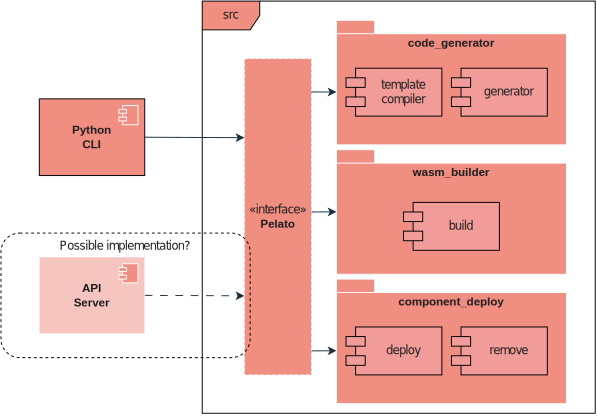
\includegraphics[width=0.8\textwidth]{img/schemi/schemi-implementazione-struttura.drawio.pdf}
    \caption{Architettura framework PELATO}
    \label{fig:pelato_architecture}
\end{figure}
\FloatBarrier

\section{Configurazione ed esecuzione framework}

In questa sezione verrà approfondita la configurazione del framework. Come già detto in precedenza il codice è scritto in Python, quindi sarà necessario avere un interprete di Python3 installato (consigliato \texttt{Python 3.12}), inoltre sarà necessario installare le librerie specificate nel \texttt{requirement.txt}. L'approccio consigliato è quello di utilizzare un virtual environment, cioè un'istanza dell'interprete Python che consente di installare le librerie localmente, senza toccare l'interprete configurato nel sistema o preoccuparsi di eventuali incompatibilità.\\
La configurazione dinamica avviene tramite variabili d'ambiente, ottenute dal sistema all'inizio di ogni esecuzione. Per facilitare il processo di configurazione è possibile creare un file \texttt{.env} situato nella cartella del framework: all'inizio di ogni esecuzione il file .env viene parsato e le variabili al suo interno vengono utilizzate per impostare il servizio.\\
All'interno della repository è predisposto il file \texttt{.env.template}, nel quale sono riportate le variabili d'ambienti impostabili e la configurazione di default, che viene mostrata nel Listing \ref{code:env}.

\begin{lstlisting}[language=bash, caption={Variabili d'ambiente per la configurazione del framework}, captionpos=b, label={code:env}]
    REGISTRY_URL=
    REGISTRY_USER=
    REGISTRY_PASSWORD=
    PARALLEL_BUILD=True
    NATS_HOST=localhost
    NATS_PORT=4222
    ENABLE_METRICS=True
\end{lstlisting}

Andiamo ad analizzarle:
\begin{itemize}
    \item \texttt{REGISTRY\_URL}, \texttt{REGISTRY\_USER}, \texttt{REGISTRY\_PASSWORD} servono per impostare le informazioni del registry in cui verranno caricate le immagini OCI dei moduli Wasm.
    \item \texttt{PARALLEL\_BUILD} abilita l'esecuzione dei container in modalità parallela.
    \item \texttt{NATS\_HOST} e \texttt{NATS\_PORT} sono utilizzati in fase di deployment e rappresentano l'istanza di NATS a cui il framework si collega per deployare le applicazioni sul cluster wasmCloud.
    \item \texttt{ENABLE\_METRICS} abilita la memorizzazione delle metriche ad ogni esecuzione del codice.
\end{itemize}

\subsection{Setup progetto}

L'utente finale, una volta configurato l'ambiente di esecuzione e impostate le variabili, per poter utilizzare il framework dovrà creare un progetto contenente:
\begin{itemize}
    \item Cartella \texttt{task} contenente i file Go in cui vengono definite le funzioni eseguite dai componenti Wasm.
    \item File \texttt{workflow.yaml} in cui inserire la configurazioni dei vari Task (per esempio nome, versione, template e nome del file Go) e sarà utilizzato dal generatore per compilare i template Jinja. Un esempio di file workflow viene mostrato nel Listing \ref{code:workflow_example}.    
\end{itemize}
Le modalità di compilazione di questi file verranno approfondite nel capitolo dedicato alla generazione del codice.

\begin{lstlisting}[language=yaml, caption={Esempio workflow.yaml}, captionpos=b, label={code:workflow_example}]
    project_name: Test_project
    tasks:
      - name: Temp sensor read
        type: producer_nats
        code: sensor_read.go
        targets:
          - cloud
          - edge
        source_topic: test_source_data
        dest_topic: test_dest_data
        component_name: temp_sensor_data
        version: 1.0.0
    ...
\end{lstlisting}

\subsection{PELATO CLI}

Come già anticipato in precedenza l'interfacciamento fra utente e framework è realizzata tramite una CLI, cioè un'interfaccia a riga di comando in grado di ricevere istruzioni e configurazioni.\\
Per invocare la CLI è sufficiente lanciare il comando \lstinline{python3 pelato.py}, che restituirà come output le varie opzioni e gli argomenti necessari, come mostrato nel Listing \ref{code:pelato_cli}.\\
\begin{lstlisting}[caption={Output Pelato CLI}, captionpos=b, label={code:pelato_cli}]
    usage: pelato.py [-h] {gen,build,deploy,remove,brush} ...
    Generate, build and deploy WASM components written in go
    
                        Command list
    gen                 Generate Go code
    build               Build WASM component
    deploy              Deploy WASM components
    remove              Remove deployed WASM components
    brush               Starts the pipeline: gen -> build -> deploy

    options:
      -h, --help            show this help message and exit
\end{lstlisting}

Ognuno di essi necessita come ulteriore argomento la path della cartella in cui sono contenuti il file \texttt{workflow.yaml} e le \texttt{task}. Nel Listing \ref{code:pelato_cli_examples} vengono riportati alcuni esempi di utilizzo.

\begin{lstlisting}[language=bash, caption={Cheatsheet comandi Pelato CLI}, captionpos=b, label={code:pelato_cli_examples}]
    $ python3 pelato.py -h      # help
    $ python3 pelato.py gen /home/lore/documents/project/   # generazione
    $ python3 pelato.py remove project/ # rimozione
    $ python3 pelato.py brush project/  # esecuzione pipeline
\end{lstlisting}

\section{Pipeline di esecuzione}

In questa sezione verrà descritta l'intera pipeline di esecuzione del framework, basandosi sui passaggi riportati nella Figura \ref{fig:pelato_pipeline}.

\FloatBarrier
\begin{figure}[h]
    \centering
    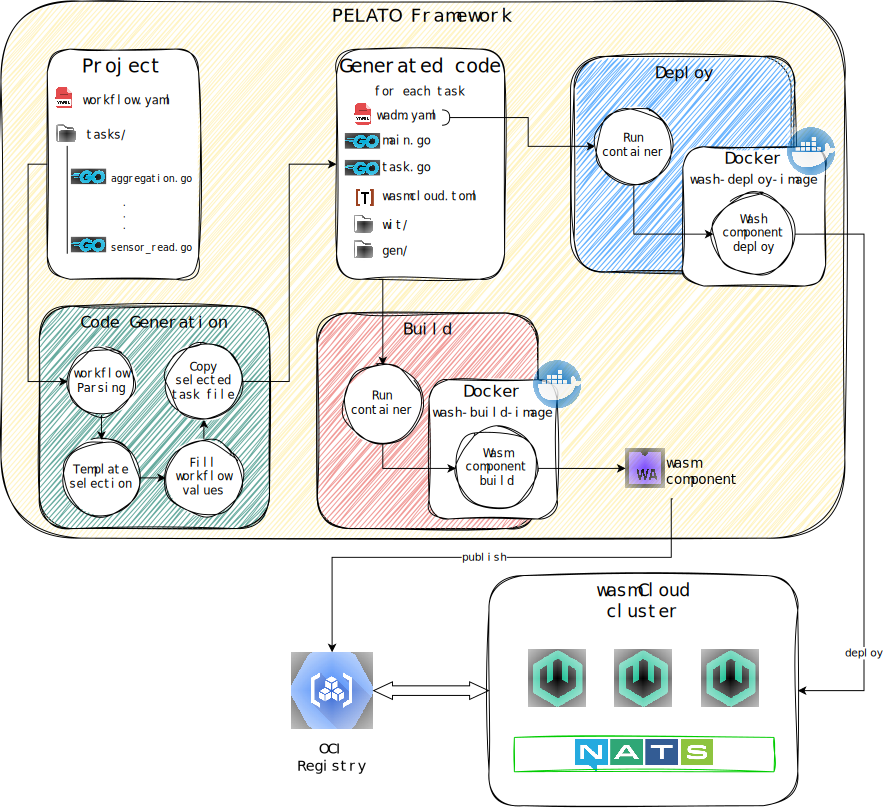
\includegraphics[width=0.9\textwidth]{img/schemi/schemi-arch-pipeline.drawio.pdf}
    \caption{Pipeline di esecuzione PELATO}
    \label{fig:pelato_pipeline}
\end{figure}
\FloatBarrier

Adesso verranno analizzati i tre componenti di esecuzione di PELATO:
\begin{enumerate}
    \item \textbf{Generazione}: in questa fase viene parsato il file \texttt{workflow.yaml} e poi utilizzato per generare i progetti Go necessari per buildare i moduli Wasm. Le configurazioni del file vengono utilizzate per selezionare il template di base, per sostituire i valori del template tramite Jinja e per identificare il file Go contenente la task. La struttura del progetto generato è mostrata nella Figura \ref{fig:pelato_pipeline} nell'area \texttt{Generated Code}.
    
    \item \textbf{Build}: questa fase si occupa di utilizzare i progetti Go generati in fase 1 e compilarli per ottenere un componente Wasm, quindi pubblicarlo come OCI artifact sul registry configurato. Queste operazioni avvengono all'interno di un container Docker nel quale sono installati tutti i tool necessari per l'operazione, come Go, TinyGo, Rust e wash.

    \item \textbf{Deploy}: è l'ultima fase della pipeline di PELATO, utilizza il manifest \texttt{wadm.yaml} generato in fase 1 per creare l'applicazione sulla piattaforma wasmCloud. Anche questa operazione avviene all'interno di un container in quanto necessita del tool wash.
\end{enumerate}

Una volta ultimato il processo, le applicazioni saranno disponibili sul wasmCloud, o lo diventeranno quando sarà presente un nodo healthy con label \texttt{host-type} corrispondente a quella selezionata dalla task.\\
La pipeline del framework è suddivisa nelle tre operazioni di generazione, build e deployment in modo che ognuna possa funzionare in modo autonomo (ovviamente se provviste delle risorse necessarie all'operazione). Inoltre, l'utilizzo di un container per le operazioni di build e deployment mira ad aumentare la compatibilità e la distribuzione del framework in modo che non sia dipendente dal sistema in cui verrà implementato: in questo progetto l'interfaccia è stata realizzata come CLI utilizzando Python, ma potrebbe essere anche esteso ad una configurazione SaaS completamente in Cloud o con approccio GitOps tramite actions e frameworks di CI/CD.\\
Tutte e tre le operazioni verranno approfondite nel dettaglio nei prossimi capitoli.